\documentclass[border=10pt]{standalone}

\usepackage{tikz}
\usepackage{tikzsymbols}
\usetikzlibrary{calc,patterns,shapes.geometric}

\def\centerarc[#1](#2)(#3:#4:#5){\draw[#1] ($(#2)+({#5*cos(#3)},{#5*sin(#3)})$) arc (#3:#4:#5);}

\begin{document}
	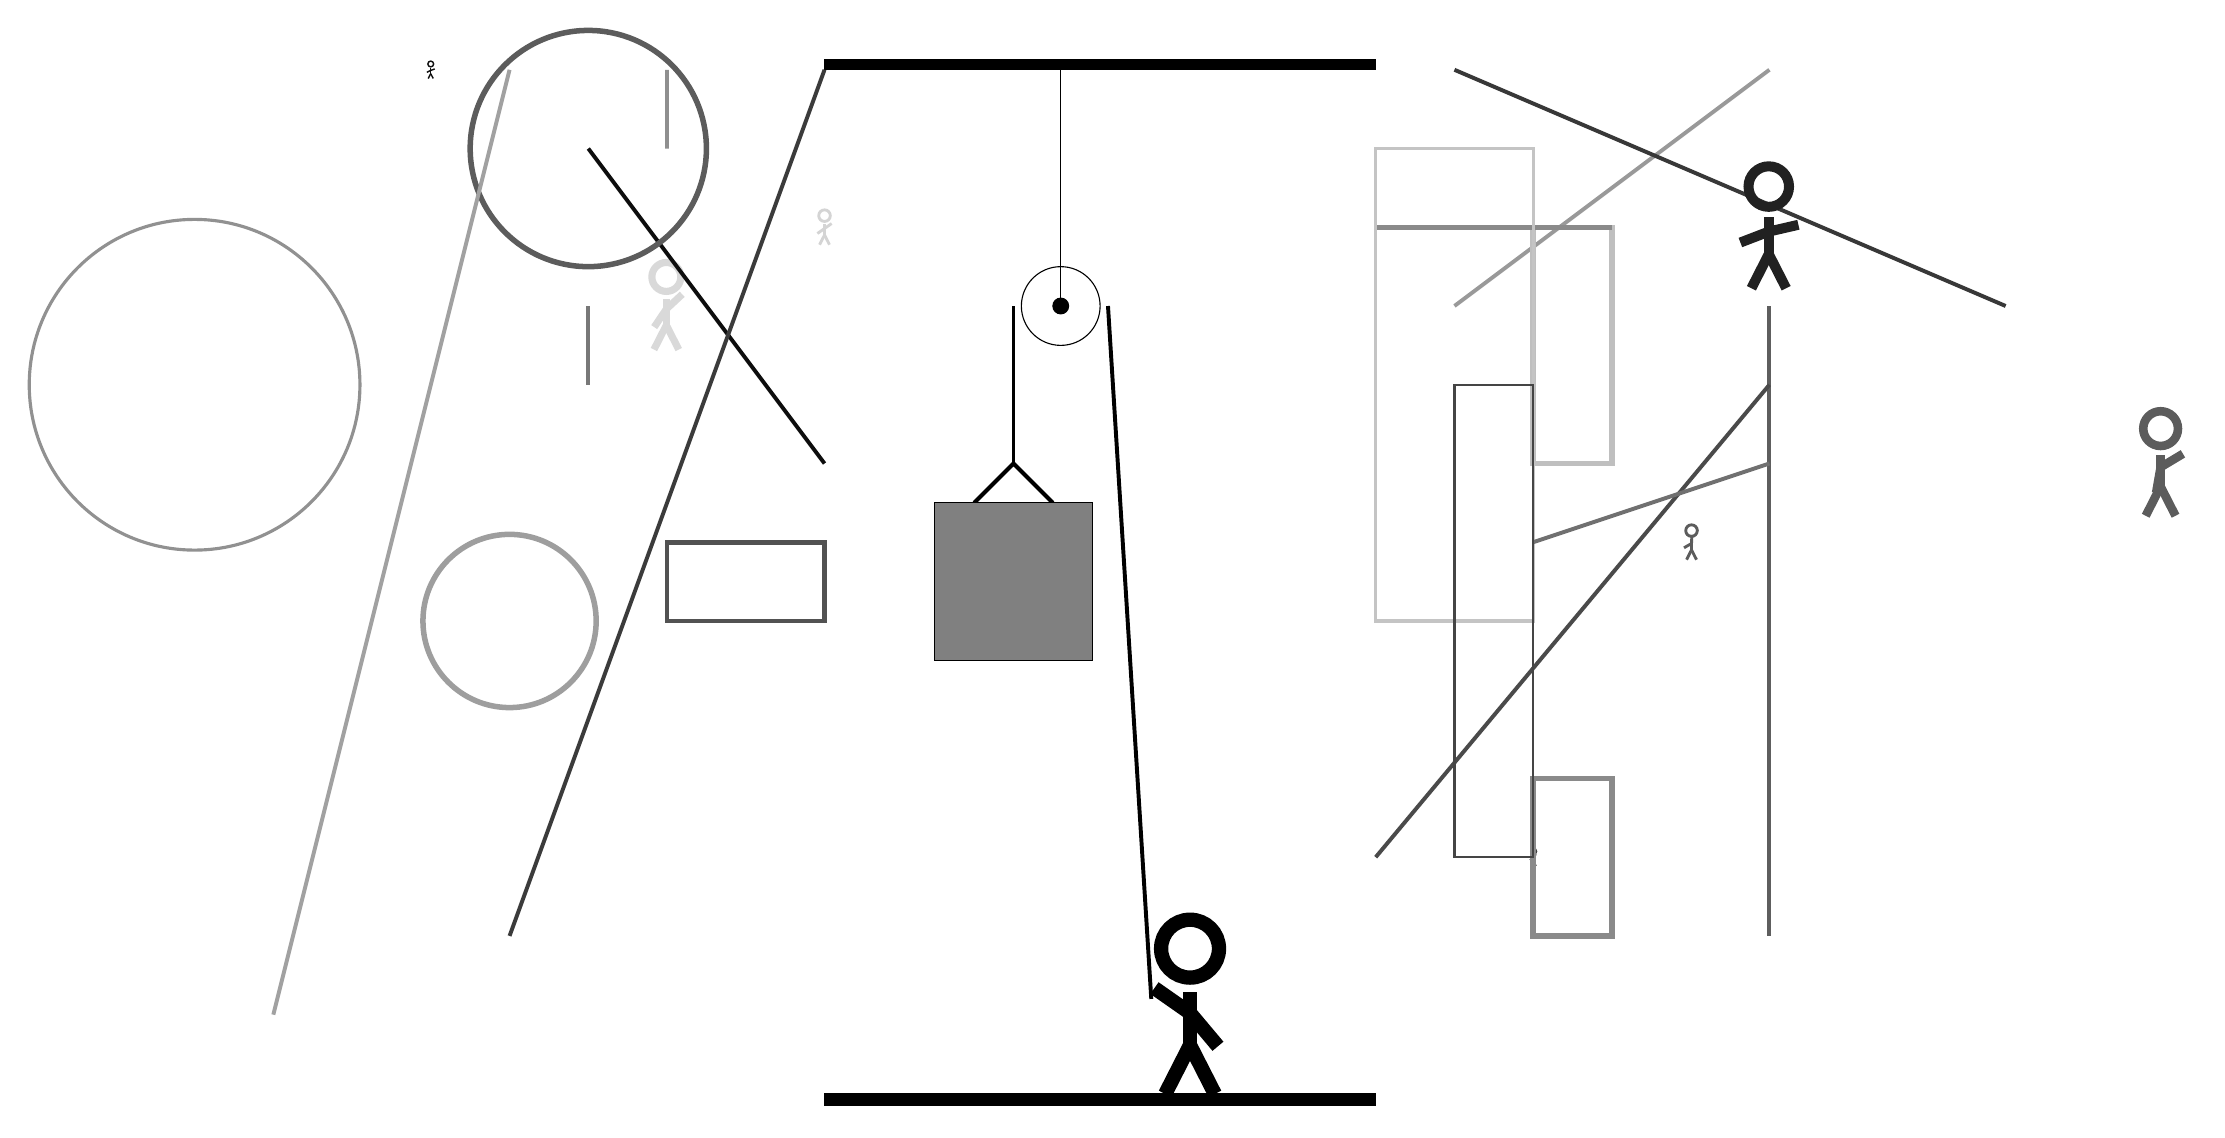
\begin{tikzpicture}
		%%%%% START %%%%%
		
		\draw[fill=black] (-2, 10) rectangle (5, 10.125);
		
		\draw (1, 7) circle (0.5);
		\draw[fill=black] (1, 7) circle (0.1);
		\draw (1, 10) -- (1, 7);
		
		\node[line width=0.4mm, color=black!15] at (-4, 7) {\Strichmaxerl[5][56][43]};
		
		\draw[line width=0.5mm, color=black!95](-5, 9) -- (-2, 5);
		\draw[line width=0.5mm, color=black!63](10, 7) -- (10, -1);
		\draw[line width=0.5mm, color=black!71](5, 0) -- (10, 6);
		
		\node[line width=0.4mm, color=black!75] at (7, 0) {\Strichmaxerl[1][28][55]};
		\draw[line width=0.6mm, color=black!68] (-4, 4) rectangle (-2, 3);
		
		\draw[line width=0.5mm, color=black!40](6, 7) -- (10, 10);
		\node[line width=0.3mm, color=black!94] at (-7, 10) {\Strichmaxerl[1][26][20]};
		\draw[line width=0.4mm, color=black!44] (-4, 10) rectangle (-4, 9);
		
		\draw[line width=0.7mm, color=black!25] (7, 8) rectangle (8, 5);
		\draw [line width=0.7mm, color=black!64](-5, 9) circle (1.5);
		\draw[line width=0.6mm, color=black!46] (5, 8) rectangle (8, 8);
		\node[line width=0.5mm, color=black!64] at (9, 4) {\Strichmaxerl[2][30][87]};
		\draw [line width=0.7mm, color=black!38](-6, 3) circle (1.1);
		\draw [line width=0.4mm, color=black!43](-10, 6) circle (2.1);
		\draw[line width=0.3mm, color=black!25] (6, 4) rectangle (6, 0);
		\draw[line width=0.5mm, color=black!77](-6, -1) -- (-2, 10);
		\draw[line width=0.4mm, color=black!23] (7, 9) rectangle (5, 3);
		\draw[line width=0.5mm, color=black!78](6, 10) -- (13, 7);
		\draw[line width=0.5mm, color=black!56](10, 5) -- (7, 4);
		\draw[line width=0.5mm, color=black!53](-5, 6) -- (-5, 7);
		
		\draw[line width=0.7mm, color=black!46] (7, 1) rectangle (8, -1);
		
		\node[line width=0.7mm, color=black!87] at (10, 8) {\Strichmaxerl[7][21][13]};
		\draw[line width=0.5mm, color=black!37](-6, 10) -- (-9, -2);
		\draw[line width=0.3mm, color=black!73] (6, 6) rectangle (7, 0);
		
		\node[line width=0.2mm, color=black!64] at (15, 5) {\Strichmaxerl[6][80][31]};
		\node[line width=0.5mm, color=black!17] at (-2, 8) {\Strichmaxerl[2][35][35]};
		
		\draw[line width=0.5mm] (-0.1, 4.5) -- (0.4, 5.0) -- (0.9, 4.5);
		\draw[fill=black!50] (-0.6, 4.5) rectangle (1.4, 2.5);
		
		\draw[line width=0.5mm] (0.4, 7) -- (0.4, 5.0);
		\centerarc[line width=0.5mm](1, 7)(0:180:0.6);
		\draw[line width=0.5mm](1.6, 7) -- (2.15, -1.8);
		
		\node at (2.6, -1.9) {\Strichmaxerl[10][-35][-50]};
		
		\draw[fill=black] (-2, -3) rectangle (5, -3.15);
		
		%%%%% END %%%%%
	\end{tikzpicture}
\end{document}